\section{Einleitung}

Im Folgenden wird beispielhaft gezeigt, wie Zitate, Bilder, Tabellen oder Quellcode in die Arbeit eingefügt werden können.

\subsection{Zitate}
Menschen, die mit ihrem IQ prahlen, sind Versager (\cite[S. 99]{hawking_1999}).

\subsection{Bilder}
\begin{figure}[H] 
    \centering
    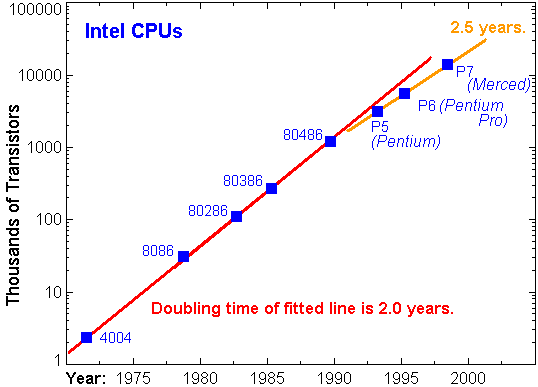
\includegraphics[width=0.5\textwidth]{figures/figure_example.png}
    \caption{Mooresches Gesetz}
\end{figure}

\subsection{Tabellen}
\begin{table}[H]
    \centering
    \begin{tabular}[H]{l|l|l}
        Bezeichnung & Kerne & TDP \\
        \hline
        Intel Core i5 & 6 & 111 W \\
        \hline
        AMD Ryzen 7 & 8 & 178 W \\
    \end{tabular}
    \caption{Prozessoren}
\end{table}


\subsection{Quellcode}
\begin{lstlisting}[language=java, caption=Hello World in Java, captionpos=b]
    class HelloWorld {
        public static void main(String[] args) {
            // Display the string.y
            System.out.println("Hello World!");
        }
    }
\end{lstlisting}
